\documentclass[10pt]{article}

\usepackage[hmargin=1.25cm, vmargin=1.5cm]{geometry} % Document margins

\usepackage{fontawesome}
\usepackage{ifsym} % Required for symbols in the colored box

\usepackage[usenames,dvipsnames]{xcolor} % Allows the definition of hex colors

\usepackage{array}
% Fonts and tweaks for XeLaTeX
\usepackage{fontspec,xltxtra,xunicode}
\defaultfontfeatures{Mapping=tex-text}
\setromanfont[Mapping=tex-text]{Hoefler Text} % Main document font
\setsansfont[Scale=MatchLowercase,Mapping=tex-text]{Gill Sans} % Font for your name at the top
%\setmonofont[Scale=MatchLowercase]{Andale Mono}
% Colors for links, text and headings
\usepackage{hyperref}
\definecolor{linkcolor}{HTML}{506266} % Blue-gray color for links
\definecolor{shade}{HTML}{F5DD9D} % Peach color for the contact information box
\definecolor{text1}{HTML}{2b2b2b} % Main document font color, off-black
\definecolor{headings}{HTML}{701112} % Dark red color for headings
\definecolor{orange}{rgb}{1,0.5,0}
% Other color palettes: shade=B9D7D9 and linkcolor=A40000; shade=D4D7FE and linkcolor=FF0080

\hypersetup{colorlinks,breaklinks, urlcolor=linkcolor, linkcolor=linkcolor} % Set up links and colors

\usepackage{fancyhdr}
\pagestyle{fancy}
\fancyhf{}
% Headers and footers can be added with the \lhead{} \rhead{} \lfoot{} \rfoot{} commands
% Example footer:
%\rfoot{\color{headings} {\sffamily Last update: \today}. Typeset with Xe\LaTeX}

\renewcommand{\headrulewidth}{0pt} % Get rid of the default rule in the header

\usepackage{titlesec} % Allows creating custom \section's

% Format of the section titles
\titleformat{\section}{\color{headings}
\scshape\Large\raggedright}{}{0em}{}[\color{black}\titlerule]

\titlespacing{\section}{0pt}{0pt}{5pt} % Spacing around titles
%FontAwesome icons
\newfontfamily{\FA}{FontAwesome Regular}
\def\twitter{{\FA \faTwitter}}
\def\phone{{\FA \faPhone}}
\def\envelope{{\FA \faEnvelope}}
\def\home{{\FA \faHome}}
\def\github{{\FA \faGithub}}
\def\globe{{\FA \faGlobe}}

\usepackage[super]{nth}

\begin{document}

\color{text1} % Sets the default text color for the whole document to the color defined as 'text1'

%----------------------------------------------------------------------------------------
%	TITLE
%----------------------------------------------------------------------------------------

\par{\centering{\sffamily\Huge Levi Lu}\\[8pt] % Your name
{\color{headings}\fontspec[Variant = 2]{Zapfino} Curriculum {Vit\fontspec[Variant = 3]{Zapfino}ae / Résumé}\\[15pt]\par} % Curriculum vitae text in the Zapfino font
	
%----------------------------------------------------------------------------------------

\begin{minipage}[t]{0.5\textwidth} % Start the left-hand side of the page
\vspace{0pt} % Trick for alignment
	
%----------------------------------------------------------------------------------------
%	WORK EXPERIENCE
%----------------------------------------------------------------------------------------

\section{Work Experience} 

%------------------------------------------------
% WORK EXPERIENCE 1
%------------------------------------------------
{\raggedleft\textsc{Summer 2014}\par}

{\raggedright\large \textbf{\textsc{The Walt Disney Company}}, Orlando\\
\textit{New Technology Group}\\[5pt]}

\begin{itemize}
	\item Responsible for building backend and data visualizing tool for dBeacon, a Disney's extension of iBeacon. \\
	{\color{Mahogany}(Neo4j, Node.js, Express.js, Angular.js, D3.js, Bootstrap)}
	\item Responsible for building an automatic bandwidth detecting system. Including databases, RESTful APIs and web UI. \\
	{\color{Mahogany}(SQL server, .NET, Angular.js, Bootstrap)}
\end{itemize}

%------------------------------------------------
% WORK EXPERIENCE 2
%------------------------------------------------

{\raggedleft\textsc{Feb 2014 -- May 2014}\par}

{\raggedright\large \textbf{\textsc{picoCTF 2014}}, United States\\
\textit{Lead Web Engineer, Game Engineer}\\[5pt]}

\textit{It’s a national wide high school hacking competition with 20000+ participants, held by CMU hacking team.}
\begin{itemize}
	\item Responsible for creating a game for the competition. \\
	{\color{Mahogany}(Impact.js, WebGL, HTML/CSS/Javascript)}
	\item Responsible for building databases and RESTful APIs. \\
	{\color{Mahogany}(Apache, MongoDB, Node.js, Express.js)}
\end{itemize}

%------------------------------------------------
% WORK EXPERIENCE 3
%------------------------------------------------

{\raggedleft\textsc{June 2012 -- June 2013}\par}

{\raggedright\large \textbf{\textsc{Papaya Mobile Inc.}}, Beijing\\
\textit{Lead Game Engineer, Web Engineer}\\[5pt]}

\begin{itemize}
	\item Building two games with over ten million downloads, \\
	as Lead Programmer : 
	\href{https://play.google.com/store/apps/details?id=com.kakapo.freeslots}{Slots Fever} and \href{https://play.google.com/store/apps/details?id=com.kakapo.bingo}{Bingo Fever}.
	\item Maintaining and adding modules to Papaya Farm, a three year old social game with over five million downloads. \\
	{\color{Mahogany}(Python)}
	\item Building web pages and maintaining Papaya SNS. \\
	{\color{Mahogany}(Python, HTML/CSS/Javascript)}
\end{itemize}

%------------------------------------------------
% WORK EXPERIENCE 4
%------------------------------------------------

{\raggedleft\textsc{July 2009 -- May 2012}\par}

{\raggedright\large \textbf{\textsc{ChinaCache}}, Nanjing / Beijing\\
\textit{Network Analyst, CDN Lab, Tsinghua University}\\[5pt]}
\begin{itemize}
	\item Responsible for building the first nationwide delay-time measuring platform in China. \\
	{\color{Mahogany}(Python, Django, Network Coordinates)}
	\item Responsible for building a streaming media platform. \\
	{\color{Mahogany}(Java/JSP, Apache)}
	\item Conducting research in “Content Delivery Network”, “Streaming Media” and “Request Routing”, intensively studying CDN, NDN and next-generation network.
\end{itemize}

%----------------------------------------------------------------------------------------	

\end{minipage} % End the left-hand side of the page
\hfill
\begin{minipage}[t]{0.44\textwidth} % Start the right-hand side of the page
\vspace{0pt} % Trick for alignment

%----------------------------------------------------------------------------------------
%	COLORED BOX
%----------------------------------------------------------------------------------------

\colorbox{shade}{\ttfamily\textcolor{text1}{
\begin{tabular}{@{} m{1cm} r m{4.8cm}}
\smash{\raisebox{-\totalheight}{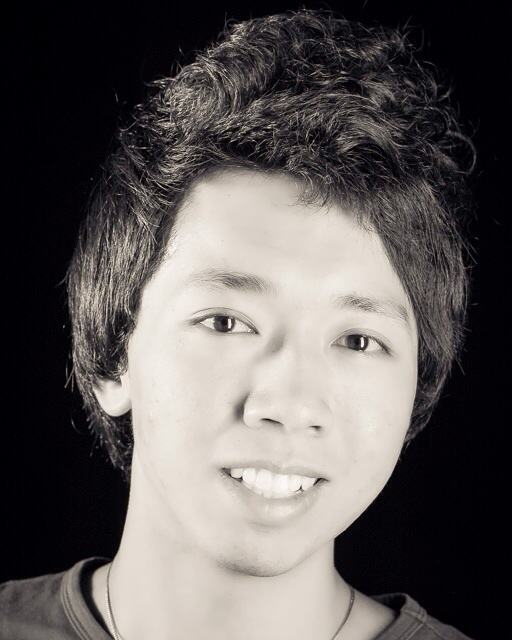
\includegraphics[width=18mm, height=22.5mm]{Xinghu.JPG}}} 
& \home & 322 Melwood Ave, PA 15213 \\ % Address
& \phone & +1~(412)~614~1371 \\ % Phone number
& \envelope & \href{mailto:xinghu1989@gmail.com}{xinghu1989@gmail.com} \\ % Email address
& \globe & \href{http://levi-lu.net}{http://levi-lu.net} \\ % Website
& \github & \href{https://github.com/xinghul}{https://github.com/xinghul} \\ % Github
\end{tabular}
}
}\\[1pt]

%----------------------------------------------------------------------------------------
%	EDUCATION
%----------------------------------------------------------------------------------------

\section{Education} 

\begin{tabular}{rl} % Start a table with two columns, one for dates and one for qualifications

%------------------------------------------------
% EDUCATION 1
%------------------------------------------------

2013 -- \textsc{Present} & \textbf{Master of Entertainment Technology} \\ 
& \textsc{Computer Science} \\ 
& \textit{Carnegie Mellon University, United States}\\
&\\

%------------------------------------------------
% EDUCATION 2
%------------------------------------------------

2008 -- 2012 & \textbf{Bachelor of Computer Science}\\
& \textsc{Computer Science} \\
& \textit{Tsinghua University, China} 
	
%----------------------------------------------------------------------------------------

\end{tabular}\\[10pt]

%----------------------------------------------------------------------------------------
%	AWARDS
%----------------------------------------------------------------------------------------

\section{Awards} 

\begin{tabular}{rl}
2012	 & \textbf{Graduate with Highest Honors}\\
& \textit{Tsinghua University}\\ \\

%------------------------------------------------

2010	 & \textbf{\nth{2} Prize of \nth{7} Challenge Cup}\\
& \textit{China association for science and technology}\\ \\

%------------------------------------------------

2007	 & \textbf{Gold Medal for HopeCup}\\
& \textit{National Mathematics Competition, China}
\end{tabular}\\[10pt]

%----------------------------------------------------------------------------------------
%	COMPUTER SKILLS
%----------------------------------------------------------------------------------------

\section{Computer Skills} 

\begin{tabular}{r l}
\textsc{Programming Languages}
& \textsc{Java/C\texttt{\#}, C/C\texttt{++}}\\
& Python, Ruby, SQL\\
& \textsc{HTML5/CSS3/Javascript}\\ 
& \\
\textsc{Operating Systems}
& Linux, Macintosh\\
& Microsoft Windows \\
& \\
\textsc{Databases}
& MongoDB, Neo4j \\
& SQL server, MySQL \\
& \\
\textsc{Platforms / Frameworks}
& Visual Studio, Unity3D\\
& NetBeans, Eclipse \\
& Node.js, .NET\\
& Angular.js, D3.js, Bootstrap \\
& \\
\end{tabular}

%----------------------------------------------------------------------------------------
%	SIDE PROJECTS
%----------------------------------------------------------------------------------------

\section{Side Projects} 
I built my own blog website from scratch:\\[2pt]
\href{http://levi-lu.net}{http://levi-lu.net} \\[2pt]
This is the place where I try out new ideas and technologies. I also built my own markdown editor to pack away articles I feel useful.

%----------------------------------------------------------------------------------------
	
\end{minipage} % End right-hand side of the page

\end{document}  